\documentclass[12pt]{article}
\usepackage[paper=a4paper,margin=1in]{geometry}
\usepackage[spanish]{babel}
\usepackage[utf8]{inputenc}
\usepackage{amsmath}
\usepackage{amssymb}
\usepackage{enumerate}
\usepackage[ruled,vlined]{algorithm2e}
\usepackage{mathtools}
\usepackage{listings}
\usepackage{tikz}
\usepackage{float}
\graphicspath{{graph/}}

\author{Ibarra Moreno Gisselle }
\title{Aceptación por Umbrales\\Heurísticas}
\begin{document}
	\maketitle
	\section{Introducción}
	
	El problema del agente viajero $TSP$ \textit{(Traveler Salesman Problem)} es un 
	problema NP-duro en el campo de optimización combinatoria que plantea la pregunta:
	Dado un subconjunto de ciudades, de las cuáles todas pueden estar o no conectadas, 
	¿Cuál es el camino más corto que pase por todas las ciudades?.
	
	El problema se puede representar como la gráfica $G$ que contiene a todas las 
	ciudades, es decir, cada $v\in V(G)$ es una ciudad y cada arista $(u,v)\in E(G)$ es 
	la distancia entre un par de ciudades, y dado un subconjunto de vértices $S$ se 
	quiere saber cuál es la trayectoria de menor costo que pase por todos los vértices de
	$S$. 
	
	Debido a que $G$ no siempre será una gráfica completa, no todas las posibles 
	permutaciones de los vértices de $S$ serán soluciones factibles y 
	detectar o descartar las soluciones no factibles puede llegar a ser complicado. 
	Por lo que para facilitar la búsqueda de una solución factible del problema, se
	utilizará la gráfica completa $G_S$ donde $V_S=S$ y $E_S=\{(u,v) \mid u,v\in S \; y 
	\; u \neq v\}$. Para calcular el peso de las aristas $(u,v)\in E_S(S)$ se utilizará la 
	siguiente función de peso aumentada:
	\[w_S(u,v)=\begin{cases}
	\text{$w(u,v)$} &\quad\text{si $(u,v)\in E$ }\\
	\text{$d(u,v)*max_d(S)$} &\quad\text{en otro caso}
	\end{cases}
	\]
	Donde $d(u,v)$ es la distancia natural y se calcula como:
	\[d(u,v)=6373000(2*arctan(\sqrt{A},\sqrt{1-A}))\]
	\[A=sin^2(\frac{lat(v)-lat(u)}{2})+cos(lat(u))(cos(lat(v)))(sin^2(\frac{lon(v)-
		lon(u)}{2}))\]
	
	Se puede notar que las aristas que no existen en $G$ tendrán un 
	peso mucho mayor que las aristas que sí están en $G$. De esta forma, para evaluar la 
	trayectoria	utilizaremos la función de costo normalizada:
	\[f(S)=\sum_{i=2}^{k}\frac{ w_S(v_{i-1},v_i)}{N(S)} \]
	
	donde $N(S)$ es el normalizador dado por la suma de los elementos de $L'$ la lista con 
	las $|S|-1$ aristas más	pesadas de $S$ tales que están en $G$:
	\[ N(S)=\sum_{d\in L'} d\]
	Esto nos facilitará encontrar soluciones factibles, ya que la suma de las distancias 
	de cualquier solución factible de $S$ será menor o igual a $N(S)$ ya que es la suma
	de las aristas de $S$ más pesadas que sí se encuentran en $G$, las soluciones no
	factibles por el contrario tendrán valores mayores a 1, ya que las aristas que no 
	se encuentren en $G$ tendrán valores enormes. 
	
	\paragraph{}
	El método más sencillo y de fuerza bruta para encontrar la respuesta a este problema
	sería haciendo todas las permutaciones posibles del conjunto de ciudades, evaluar
	el costo de las trayectorias y regresar la de menor costo (la cuál podría no ser
	factible, si no existiera ninguna trayectoria). Esto es terriblemente costoso 
	computacionalmente (en memoria y tiempo), y tomaría tiempo $O(n!)$ por lo que para 
	un conjunto de ciudades grande, este algoritmo no terminaría.
	
	Por esto, se han creado diferentes algoritmos y heurísticas que encuentran
	aproximaciones al camino más corto (si es que se conoce) o caminos óptimos 
	utilizando la menor cantidad de recursos y con ejecuciones rápidas.
	
	\paragraph{}
	La heurística utilizada en este reporte es una variante del Recocido Simulado 	\textit{(Simulated Annealing)} llamada Aceptación por Umbrales (\textit{Threshold 
	Acceptance)}. El recocido simulado es una heurística inspirada en la técnica 
	metalúrgica del recocido, esta se basa en calentar y enfriar de manera controlada 
	metales, de manera que dependiendo de la velocidad del enfriamiento se obtendra un metal de mejor o peor calidad.
	
	Esta heurística depende fuertemente de la temperatura, es decir, las soluciones se
	verán afectadas por el tamaño de la temperatura inicial y que tan rápido se enfríe.
	Normalmente utiliza como condición de término que la temperatura llegue a un valor 
	$\epsilon$ que es un cero virtual.
	
	El pseudocódigo del recocido simulado clásico se puede ver en la siguiente figura:
	
	\begin{algorithm}[H]
		\SetAlgoLined
		\KwOut{$s$ solución inicial, $T$ temperatura inicial}
		\KwIn{$s$ solución encontrada}
		\While{$T \ge \epsilon$}{
			$s' \gets vecino(s)$\;
			$s \gets probabilidadAceptar(s',s,T)$\;
		}
		\Return{$s$}
		\caption{Recocido Simulado}
	\end{algorithm} 
	
	\paragraph{Algunas observaciones importantes sobre esta heurística:}
	\begin{itemize}
		\item Cuando la temperatura inicial $T$ es un valor pequeño y $\epsilon$ es muy 
		pequeña, la	heurística funciona igual a una búsqueda local como Descenso de Colinas \textit{(Hill Descending)}, lo que puede provocar que se quede en un
		mínimo local. Esto sucede ya que cada que la heurística 
		genera una nueva solución, puede empeorar dependiendo de la temperatura actual, 
		con una temperatura muy cercana a 0 el algoritmo no encontrará soluciones que 
		puedan empeorar notablemente.
		
		\item Cuando la temperatura inicial $T$ es muy grande, en las primeras 
		iteraciones el algoritmo dará mucho saltos entre mejores y peores soluciones.
		
		\item Si el algoritmo utiliza un factor de enfriamiento que disminuye la 
		temperatura muy rápidamente, las soluciones no serán muy buenas, debido a que 
		el algoritmo terminará con pocas iteraciones y no podrá buscar lo suficiente.
		
	\end{itemize}

	La variante de Aceptación por Umbrales, calcula lotes de soluciones $aceptadas$ 
	dentro de un umbral determinado por:
	\[f(s') \leq f(s)+T\]
	Además, cada solución nueva $s'$ es elegida de forma aleatoria uniforme de los
	vecinos de la solución $s$. En la siguiente figura podemos ver el pseudocódigo:
	\begin{algorithm}
		\SetAlgoLined
		\KwOut{$s$ solución inicial, $T$ temperatura inicial}
		\KwIn{$s$ solución encontrada}
		$p \gets 0$\;
		\While{$T > \epsilon$}{
			$q\gets \infty$\;
			\While{$p\le q$}{
				$q \gets p$\;
				$p,s \gets calculaLote(T,s)$\;
			}
		$T\gets \phi T$
		\Return{s}
		}
	\caption{Aceptación por Umbrales}
	\end{algorithm}

	\begin{algorithm}
		\SetAlgoLined
		\KwOut{$s$ solución inicial, $T$ temperatura inicial}
		\KwIn{$s$ solución encontrada}
		$c \gets 0$\;
		$r \gets 0.0$\;
		\While{$c<L$}{
			$s' \gets vecino(s)$\;
			\If{$f(s') \le f(s)+T$}{
				$s \gets s'$\;
				$c\gets c+1$\;
				$r \gets r+1$\;
			}	
		}
		\Return{$r/L,s$}
		\caption{$calculaLote$}
	\end{algorithm}
	
	\section{Tecnologías Utilizadas}
	
	Se utilizó el lenguaje de programación Nim para implementar la heurística. Nim es un
	lenguaje completamente compilado, multiparadigma, de propósito múltiple con tipado
	estático.
	
	El compilador genera código optimizado en C lo que hace el código bastante rápido, además, es muy sencillo de configurar y usar. El compilador también puede generar
	código en C++ y JavaScript.
	Además, tiene un recolector de basura, por lo que el programador no tiene que
	encargarse manualmente del manejo de memoria.
	
	La sintáxis de Nim es fácil de entender y aprender ya que es muy similar a la de Python, lo que hace el código muy fácil de leer. Por esta misma propiedad, es muy
	fácil pasar pseudocódigo a código en Nim.
	
	Además generar la documentación de código en Nim es muy sencillo y rápido, a la vez que la documentación generada es muy estética y fácil de entender.
	
	Por estas razones se decidió utilizar Nim para implementar la heurística de 
	Aceptación por Umbrales.
	
	
	\section{Diseño en la Implementación de la Heurística}
	\paragraph{Diseño de las Clases:}
	Utilizando el paradigma de Orientación a Objetos, se implementaron dos clases para 
	modelar las principales estructuras del problema: la Gráfica y las Soluciones.
	
	\begin{enumerate}
		\item \textbf{Gráfica}
		\begin{enumerate}
			\item \textit{Atributos:}
		\begin{itemize}
			\item \textbf{cities:} Una matriz nxn que almacena una tupla con la 
			distancia entre dos ciudades y un bool que indica si la conexión existe en G.
			\item \textbf{dim: }La dimensión de la matriz.
		\end{itemize}
		\item\textit{Métodos Principales:}
		\begin{itemize}
			\item \textbf{initGraph: }
			Para construir la gráfica se utiliza una base de datos que almacena 1092 
			ciudades con sus latitudes y longitudes, junto con las conexiones existentes 
			entre ciudades.
		Cada conexión entre dos ciudades $i,j$ en la base de datos se guarda en la matriz como $(w(i,j),true)$ y en el caso de no encontrarse la conexión se guardará en la
		matriz $(d(i,j),false)$ es decir, se guarda la distancia natural. 
	\end{itemize} 
	\end{enumerate}
		\item \textbf{Solución}
		\begin{enumerate}
		\item \textit{Atributos:}
	\begin{itemize}
		\item\textbf{cities:} La permutación, que es una lista con los índices que 
		representan cada ciudad.
		\item \textbf{norm: }El normalizador del conjunto de ciudades en la solución.
		\item \textbf{maxD: } La distancia máxima entre ciudades de la solución que 
		exista en la gráfica.
		\item \textbf{c: } El costo de la solución actual.
	\end{itemize}
	\item \textit{Métodos principales:}
	\begin{itemize}
		\item \textbf{initSolution:} Inicializa la solución guardando la permutación 
		inicial de ciudades, luego calcula y guarda el normalizador, la distancia máxima
		y el costo de la permutación. Se debe notar que el normalizador y la
		distancia máxima siempre son los mismos por más intercambios que sufra la 
		permutación, por lo que sólo se calcularán una vez para optimizar el tiempo 
		que tardará el algoritmo.
		\item \textbf{randomNeighbor:} Calcula el valor de un vecino e indica que índices
		se deben intercambiar en la permutación para obtener el costo de este. Este 
		método es una optimización para calcular el costo de un vecino sin
		ocupar memoria en generarlo y tomando tiempo constante , esto
		se puede lograr ya que un vecino de la solución es sólo el intercambio entre dos
		índices de la permutación, por lo que a lo más sólo 4 conexiones se ven afectadas
		en el costo, por lo que se deben restar las conexiones conectadas a los índices
		anteriores y sumar las nuevas conexiones formadas por el intercambio. 
		\item \textbf{swap:} Intercambia los elementos en los índices $i,j$ de la 
		permutación y asigna el nuevo costo de la solución. Este método será muy útil 
		para cuando la heurística encuentre una	solución que caiga dentro del umbral, de
		esta forma sólo tendrá que intercambiar los valores y actualizar el costo.
		\item \textbf{normalizer: } Calcula en normalizador de S.
		\item \textbf{maxDistance: } Calcula la distancia máxima en S.
		\item \textbf{cost: } Calcula el costo de la solución.
	\end{itemize}
	\end{enumerate}
	\end{enumerate}
	
	Así ya tenemos las clases necesarias para el algoritmo.
	
	\paragraph{Módulos:} 
	Además de los módulos que contienen a las clases, se tienen el módulo principal, un
	módulo auxiliar para calcular todo lo relacionado a las distancias y el módulo con
	la heurística principal junto con la metaheurística para calcular una temperatura
	inicial óptima.
	
	El módulo auxiliar, contiene los procedimientos relacionados con las distancias, 
	como son la consulta a la base para obtener el valor de las conexiones entre pares
	de ciudades, la consulta para obtener las longitudes y latitudes de las ciudades y el
	cálculo de la distancia natural. Este módulo es utilizado por el módulo de la clase
	gráfica para construir la matriz de adyacencia.
	
	El módulo más importante es el que contiene los procedimientos necesarios para llevar
	a cabo la heurística. En este módulo vienen implementados los pseudocódigos vistos
	en la introducción de este documento, es decir, la heurística de aceptación por 
	umbrales y el algoritmo auxiliar de $calculaLote$. Además se tiene un algoritmo para
	calcular la temperatura inicial óptima para una solución.
	
	
	\section{Resultados}	
	
	La heurística se probó con dos instancias, una de 40 ciudades y una de 150 ciudades.
	En la siguiente tabla se pueden ver los mejores resultados obtenidos después de 
	ejecutar la heurística con 1000 semillas para cada instancia:
	
	\begin{table}[H]
		\centering
		\caption{Las mejores soluciones encontradas en 1000 semillas}
		\begin{tabular}{|p{0.12\textwidth}|p{0.09\textwidth}|p{0.08\textwidth}|p{0.20\textwidth}|p{0.20\textwidth}|p{0.21\textwidth}|}
			\hline 
			\textbf{Instancia} & \textbf{Semilla} & $\displaystyle \epsilon $ & \textbf{Temperatura Inicial} & \textbf{Costo Inicial} & \textbf{Costo final} \\
			\hline 
			{\small data40.txt} & {\small 581} & {\small 0.0001} & {\small 342344.5816040039} & {\small 305585.454990047} & {\small 0.2191942637507401} \\
			\hline 
			{\small data40.txt} & {\small 712} & {\small 0.0001} & {\small 352562.8380775452} & {\small 305585.454990047} & {\small 0.2192475222521434} \\
			\hline 
			{\small data40.txt} & {\small 939} & {\small 0.0001} & {\small 344503.9381980896} & {\small 305585.454990047} & {\small 0.217571010694417} \\
			\hline 
			{\small data150.txt} & {\small 30} & {\small 0.0001} & {\small 119984.2529296875} & {\small 6152051.625245280} & {\small 0.1599342998110141} \\
			\hline 
			{\small data150.txt} & {\small 102} & {\small 0.0001} & {\small 120851.5625} & {\small 6152051.625245280} & {\small 0.1539785509479406} \\
			\hline 
			{\small data150.txt} & {\small 752} & {\small 0.0001} & {\small 123000.0} & {\small 6152051.625245280} & {\small 0.1498899901866556} \\
			\hline
		\end{tabular}
		
	\end{table}
	
	
	A continuación se muestran las gráficas de la evolución de la ejecución que encontró 
	el mejor costo para las dos instancias probadas.
	En las gráficas se hace la comparación entre la mejor solución encontrada y la
	solución actual al final de la generación de un lote.
	
	\begin{figure}[H]
		\centering
		\caption{Gráfica de evolución de la instancia de 40}
		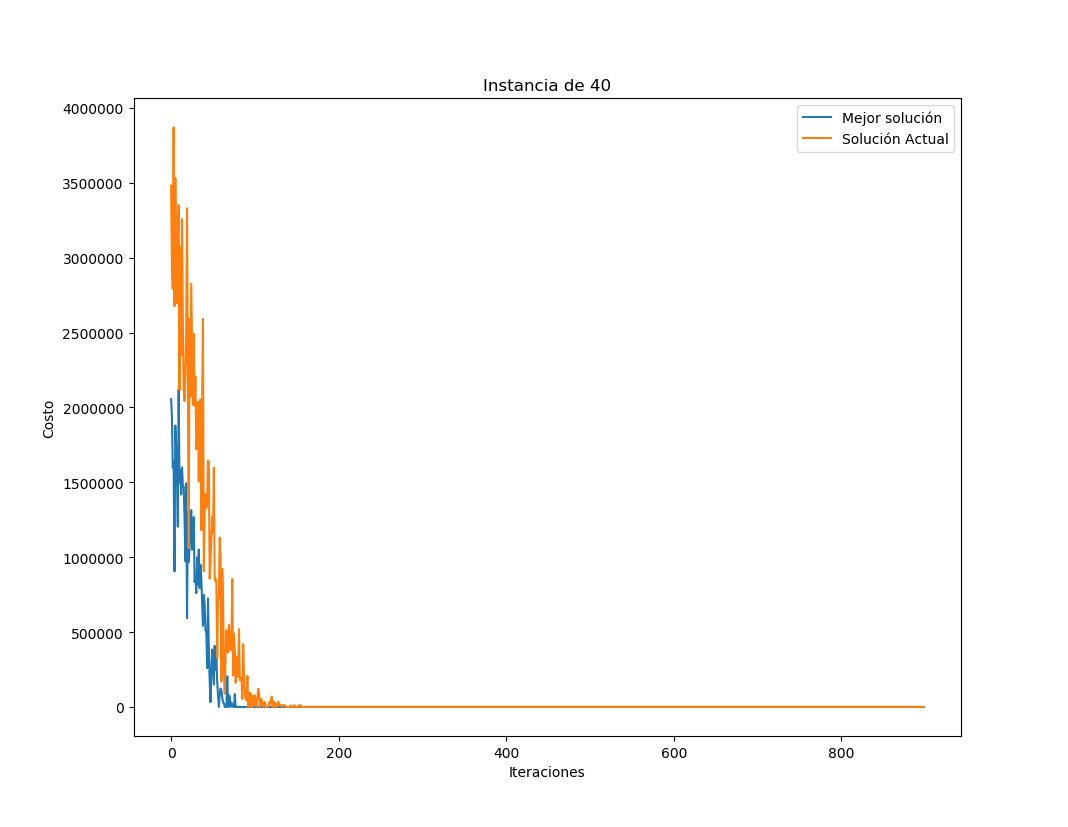
\includegraphics[scale=0.6,width=12cm]{I40_1.png}
	\end{figure}
	\begin{figure}[H]
		\centering
		\caption{Convergencia en la gráfica de evolución de la instancia de 40}
		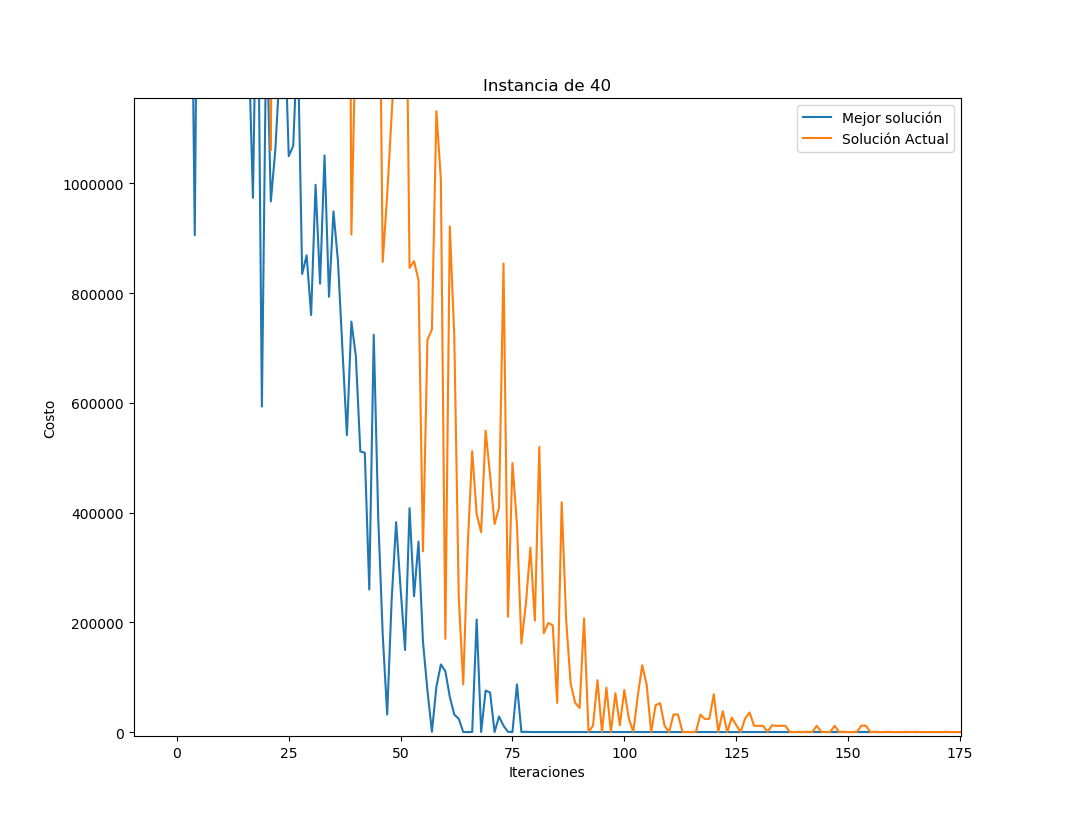
\includegraphics[scale=0.6,width=12cm]{I40_2.png}
	\end{figure}
	\begin{figure}[H]
		\centering
		\caption{Gráfica de evolución de 200 iteraciones de la instancia de 40}
		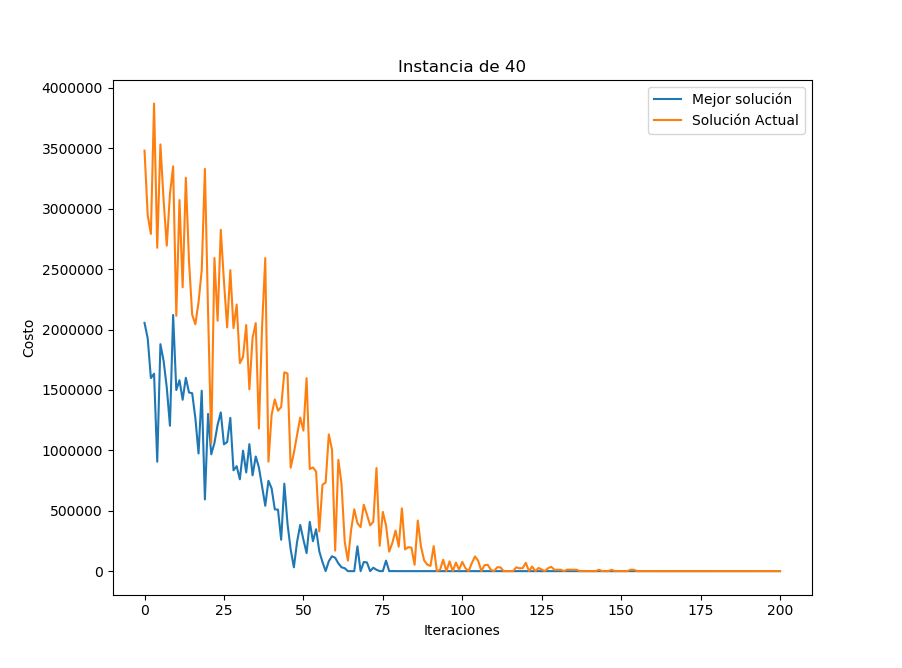
\includegraphics[scale=0.6,width=12cm]{I40_3.png}
	\end{figure}
	\begin{figure}[H]
		\centering
		\caption{Gráfica de evolución de la instancia de 150}
		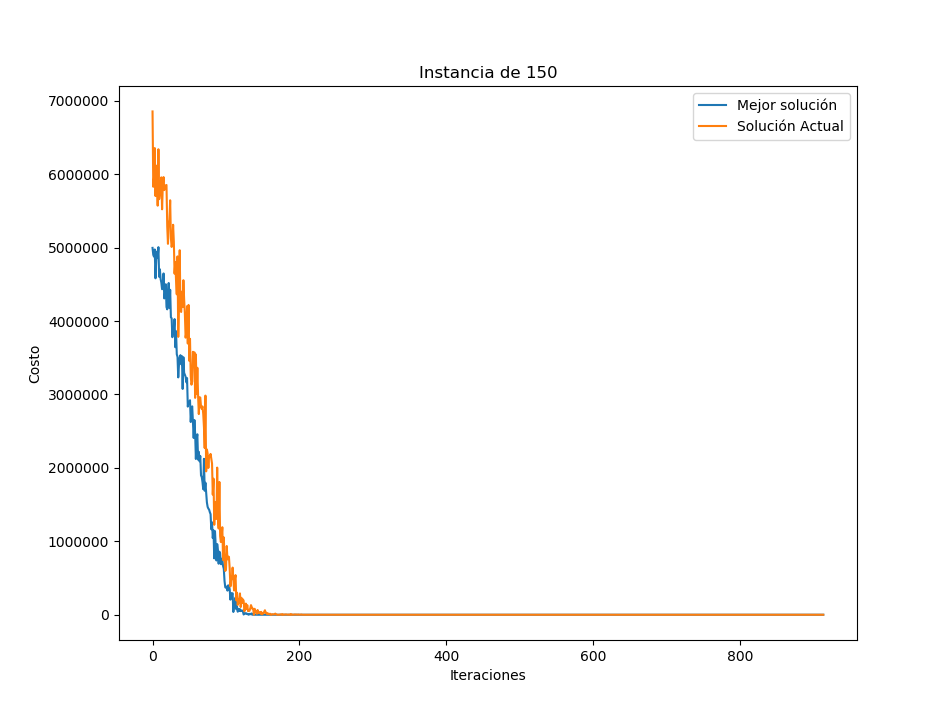
\includegraphics[scale=0.6,width=12cm]{I150_1.png}
	\end{figure}
	\begin{figure}[H]
		\centering
		\caption{Convergencia de la gráfica de evolución de la instancia de 150}
		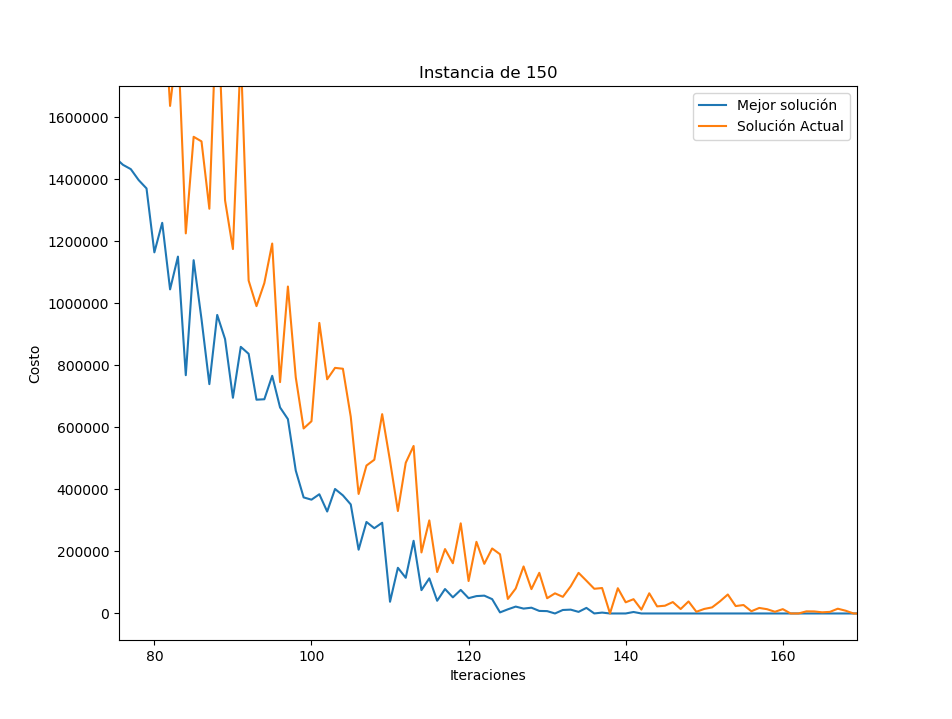
\includegraphics[scale=0.6,width=12cm]{I150_2.png}
	\end{figure}
	\begin{figure}[H]
		\centering
		\caption{Gráfica de evolución de 200 iteraciones de la instancia de 150}
		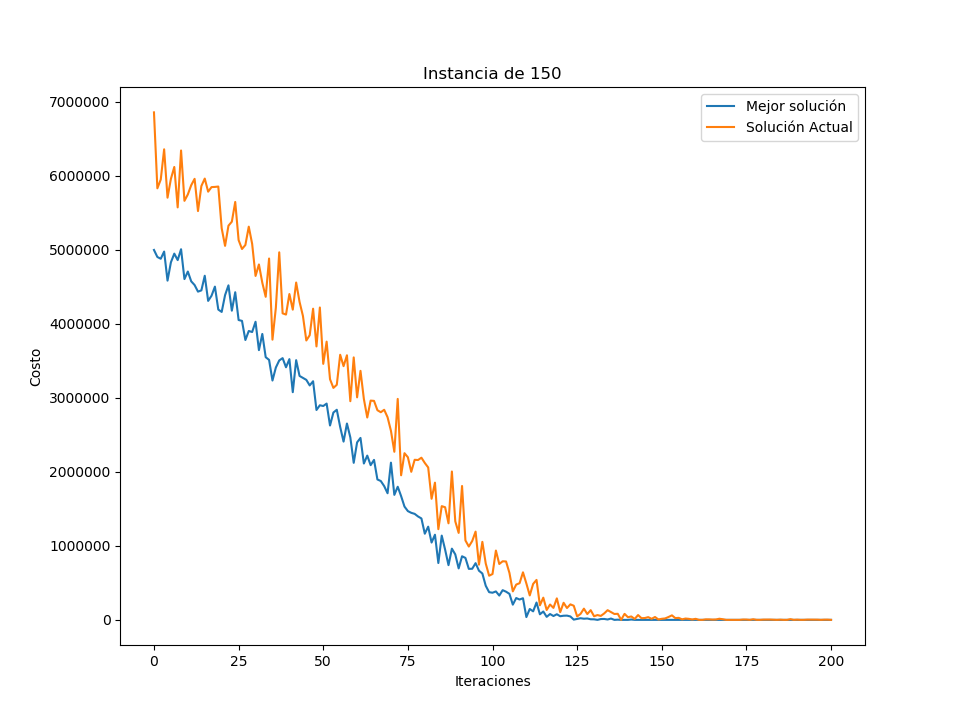
\includegraphics[scale=0.6,width=12cm]{I150_3.png}
	\end{figure}
	\section{Conclusiones}
	
	Los resultados obtenidos para las dos instancias fueron bastante satisfactorios, se lograron encontrar las soluciones óptimas y la ejecución del algoritmo es bastante 
	rápida,	ya que para la mayoría de las semillas la ejecución tarda menos de 30 
	segundos.
	 
	\section{Bibliografía}
	
	\begin{itemize}
		\item Artículo TSP:  https://www.quantamagazine.org/computer-scientists-break-traveling-salesperson-record-20201008/https://arxiv.org/abs/2007.01409
		\item  Documentación de Nim : https://nim-lang.org/
		\item Documento hoc.pdf del Profesor Canek Peláez Valdés
		\item Presentación 07\_RecocidoSimulado.pdf del Profesor Oscar Hernández 
		Constantino 
	\end{itemize}
	
\end{document}